\documentclass[../main.tex]{subfiles}

\begin{document}

\section{Elementos sometidos a compresión}

\subsection{Resistencia de diseño a compresión}

La resistencia de diseño para pandeo flexional de barras comprimidas axialmente
se determina de la siguiente forma:

\begin{align*}
  \phi_c * P_n
.\end{align*}

Donde $\phi_c=0.85$ y $P_n$ es la resistencia nominal en kN, dado que $P_n = F_{cr}*A_g*10^{-1}$

La tensión crítica de pandeo $F_{cr}$ dependiendo del factor de esbeltez, que 
se calcula como:

\begin{align*}
  \lambda_c = \frac{1}{\pi}*\frac{k*L}{r}*\sqrt{\frac{F_y}{E}} \tag{Esbeltez} \label{esbeltez}
.\end{align*}

Vemos, que para un mayor radio de giro, tendremos menor esbeltez, que nos permite
cargar más la columna. Esto lo podemos ver al calcular $F_{cr}$, que se calcula
de la siguiente forma:

\begin{align*}
  \begin{cases}
    \lambda_cd \leq 1.5 \rightarrow F_{cr} = 0.658^{\lambda^2_c}*F_y \\
    \lambda_cd \geq  1.5 \rightarrow F_{cr} = \frac{0.877}{\lambda^2_c}*F_y
  \end{cases}
.\end{align*}

La variación dependiendo se debe a la existencia de \textbf{tensiones residuales}
que pueden hacer que elementos entren en fluencia antes de lo previsto. Por eso
es necesario para esbelteces bajas tener especial cuidado.

\subsection{Longitud efectiva de una barra comprimida}

El \textbf{factor de longitud efectiva} $k$ se debe determinar de acuerdo con lo
especificado en el Capitulo C, Sección C.2 del reglamento CIRSOC 301. Los valores
presentados en \Cref{fig:long-efectiva}, se pueden ver valores recomendados en 
casos donde no se usen lo nomogramas (recomendado).

\begin{figure}[ht]
  \centering
  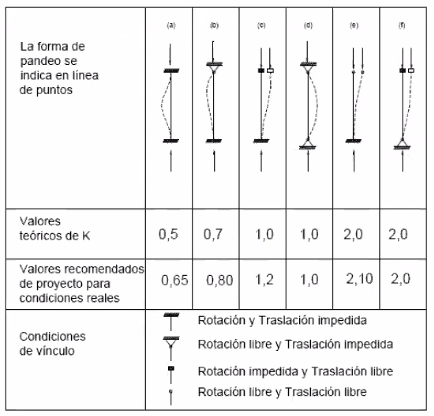
\includegraphics[width=0.8\textwidth]{../images/20210419/long-efectiva}
  \caption{Valores recomendados para k}
  \label{fig:long-efectiva}
\end{figure}

El uso de nomogramas depende de si tenemos estructuras desplazables o indesplazables,
donde se obtienen valores de $G_a$ y  $G_b$, que salen de la siguiente formula:

\begin{align*}
  G = \frac{\Sigma (I_c / L_c}{\Sigma I_g / L_g}
.\end{align*}

Donde se consideran las rigideces que vienen de las columnas y de las vigas.

Este punto es crítico, ya que de él dependen todos los valores y fuerzas admisibles 
a compresión.

\subsection{Clasificación de secciones}
Las secciones pueden ser compactas, no compactas y con elementos esbeltos.
Es importante saber cuando los elementos son \textbf{esbeltos}, ya que se pueden
dar pandeos o abollamientos en los lados o alas de la columna. Esto queda claro
en la \cref{fig:abollamiento}.

\begin{figure}[ht]
  \centering
  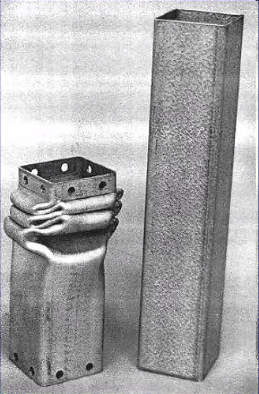
\includegraphics[width=0.8\textwidth]{../images/20210419/abollamiento}
  \caption{Pandeo local.}
  \label{fig:abollamiento}
\end{figure}  

La forma de calcular si un elemento es esbelto o no se hace desde la Tabla B.5.1.
del reglamento CIRSOC 301. Esta presenta varios casos, donde describe el elemento
y da la forma para considerar el tipo de elemento. 

En caso de que los elementos no son esbeltos, podemos seguir utilizando las
formulas a utilizar son las dadas, y caso contrario se lo deberá afectar por un
coeficiente $Q$ que penalizará esta condición.







\end{document}
